\chapter{\label{sec:casestudy}Literature Review}
\section{Introduction to Quantum Computing}
In a society where the development of technology has greatly impacted our lives it is interesting to think that not so long ago, in 1936, the idea of a computer or a "Turing machine" was an abstract concept devised by Alan Turing~\citep{Turing1937OnEntscheidungsproblem,Nielsen2010QuantumInformation}. The basic idea of the machine is is an infinite tape of cells and a tip head moves along the tape with the ability to modifying and read out the cell contents. Therefore for any problem by programming a series of instructions to the machine can simulate the outcome. Many problems are efficiently solvable using a deterministic Turing machine. However, complexity classes were devised as a way to assess the difficulty of a problem based on the resources, space or time, required for simulation. For $\bm{P}$ problems the solution can be gained in polynomial time, which means time is a polynomial function of the size of input bits, n. However, there are a range of algorithms where the computational time required scales exponentially and means as $n$ increases the computation quickly becomes impracticable~\citep{talbot_welsh_2006}.

Furthermore, the field of quantum mechanics was born in 1900 following Planck's solution to the spectral energy density of blackbody radiation~\citep{Maxplanck}. This lead to the idea of quantisation where Einstein proposed the idea of energy quanta and postulated that energy is absorbed or emitted in discrete amounts~\citep{doi:10.1002/andp.19053220607}. This idea was verified by the famous photoelectric effect experiment~\citep{0143-0807-32-4-018}. In the years following applications and experimental studies of quantum mechanics theory grew, particularly following the development of the maser~\citep{PhysRev.99.1264}. Additionally, the development of the transistor in 1958 lead to the first integrated circuit which was the revolutionized the study of computer science ~\citep{Arns1998TheTransistor}. 

Moore's prediction of the population increase by reduction in the transistor size has held correct for the past 30 years~\citep{Moore1965CramingCircuits}. However, continuing to increase computational power by the scaling down the transducer size is reaching the fundamental limit where quantum effects of electrons dominate circuit operation. Investigation of algorithms to efficiently solve problems that are outwidth $\bm{P}$-space lead to the classification of the bounded error, quantum, polynomial time (BQP) complexity class. BQP includes all problems which are solvable using a quantum computer. Computational power is increased $\bm{(1)}:$ due to the ability to store information in a superposition of bit states, $\epsilon \left \{ 0,1 \right \}$ known as a qubit: 

\begin{equation}
\label{eq:qubit}
\ket{\Psi} = \alpha \ket{0} + \beta \ket{1},  
\end{equation} 

\noindent where $\alpha, \beta$ are complex probability amplitudes, and $\bm{(2)}:$ the ability to entangle qubits ~\citep{Nielsen2010QuantumInformation}. For example the factorization problem Shor's algorithm~\citep{doi:10.1137/S0097539795293172} computes the result in polynomial time and Grover's search algorithm provides quadratic speed up compared to classical computation~\citep{Grover:1996:FQM:237814.237866}. Additionally, in 1982 Feynman first introduced the idea that to simulate quantum behaviour, this required a universal computer which is also quantum in nature~\citep{Feynman1982}. 

In the pursuit to build a quantum computer the system to provide the basic quantum unit, satisfying the DiVencenzo criteria~\citep{Divincenzo2000TheComputation}, is an active area of research. There is a large variety of systems being investigated including: atoms, ions, photons, superconducting circuits (SC), quantum dots and atomic impurity spins in solids ~\citep{0034-4885-74-10-104401,10.1038/nature07129,MORTON2018128}.   
  


\section{Prospects of Rare-earth Doped YSO for Quantum Computing}
Distributed quantum computing is the scheme were a large scale quantum computer is sectioned into nodes connected via optical channels~\citep{DiVincenzo255}. The separation of quantum nodes is limited by light attenuation for distribution $>$100 km and the no-cloning theorem which prevents classical amplification of entangled photons~\citep{Duan2001Long-distanceOptics}. This principle naturally leads to the hybrid quantum computing approach where disparate qubits are used to their individual advantage to form either local processors or memory qubits in each node~\citep{nature07127}. Scalable solid state devices such as SC circuits, SC resonators~\citep{Houck2009} and donor electron spins in doped solids \citep{doi:10.1146/annurev-conmatphys-062910-140514} provide fast (ns) gate manipulation and microwave regime readout. These systems provide promising candidates to provide processor qubits. Conversely, their ability to store information is limited by their short ($\mu$s) coherence times. Thus it is advantageous for memory qubits to also provide coherent microwave-to-optical conversion as means of interfacing photonic and solid state qubits. Currently quantum repeaters systems are focused on cavity QED approaches where the memory qubit is provided by: NV centers in diamond~\citep{PhysRevA.92.020301}, Rydberg atoms~\citep{PhysRevA.96.013833} or rare-earth (RE) doped crystals~\citep{PhysRevB.84.060501}. Details of the crystal structure and energy level splitting of RE doped YSO is detailed in Section.~\ref{sec:YSO}.  

Replacing yttrium atoms with RE ions results in small inhomogeneous broadening of the microwave and optical transitions. Thus RE doped YSO presents a promising platform for hybrid quantum computing where the host lattice has a low nuclear spin abundance~\citep{PhysRevB.97.064409}. The demonstration of a coherence time of 370 minutes for the nuclear spin of $^{151}$Eu doped Y$_{2}$SiO$_{5}$~\citep{nature14025} at 2 K motivates the study of RE ions for coherent quantum information storage applications. This system provides the longest measured coherence time of a quantum memory system with optically accessible transitions. This result is achieved by a reduction in the decoherence of the +3/2 $\leftrightarrow$ -3/2 hyperfine transitions firstly reducing the sensitivity to fluctuations of the magnetic field $\bm{B_{0}}$, reducing the spin-reconfiguration rate and lastly the inclusion of the KDD$_{x}$ pulse sequence. Due to the zero-field splitting of hyperfine states, operation at the zero first-order Zeeman (ZEFOZ) magnetic field produces hyperfine clock transitions the expected ideal decoherence rate is 2.9$\time 10^{-2}$ s$^{-1}$. 

A significantly smaller decoherence rate is observed for the case where the pulse separation time  $\tau$ of the Hahn echo sequence is considerably shorter than the phase memory time, $T_{M}$~\citep{PhysRev.168.370}. The "froze core" effect~\citep{PhysRevB.91.214303} reduces the spin flipping rate of the Yttrium nuclear spins around an Eu ion due the hyperfine interaction with the magnetic moment of the unpaired electron in a large magnetic field as shown in Fig.~\ref{fig:frozencore}. The nuclear dipolar interaction resulting in a fluctuating magnetic field is therefore reduced~\citep{RevModPhys.79.1217}. Further extension of the spin coherence time was successfully achieved using the KDD$_{x}$ pulse sequence. This sequence provides dynamical decoupling from the environment to provide protection from the environmental induced dephasing using a series of refocusing pulses~\citep{PhysRevLett.106.240501}. 

\begin{figure}[h]
\centering
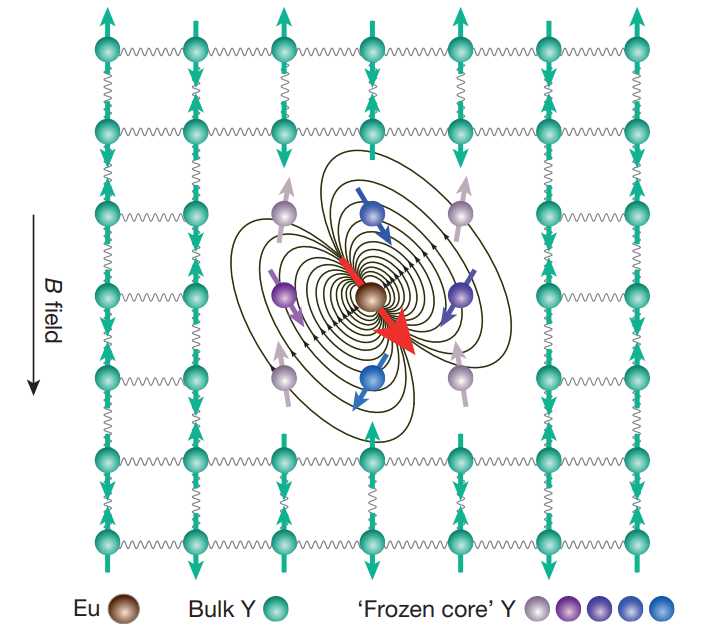
\includegraphics[height=0.32\textwidth,keepaspectratio]{frozencore}
\caption{\label{fig:frozencore} The "frozen core" effect where the large electron dipole moment (red arrow) of the Eu ion induced by an external magnetic field modifies the Larmor frequency of Yttrium spin procession such that Yttrium ions in the frozen core cannot swap spin with the bulk Yttrium nuclei ~\citep{nature14025}.}
\end{figure}


Including microwave electron paramagnetic resonant transitions, RE ions have near infra-red optical transitions~\citep{PhysRevB.94.155116}. Therefore, the active research investigates the ability to couple RE doped crystals to SC resonators. Strong coupling is achieved between SC niobium chip and Er$^{3+}$ doped Y$_{2}$SiO$_{5}$ has been achieved~\citep{PhysRevLett.110.157001}. The SC device contains 9 $\approx$50 GHz element resonators which is connected by glue to two RE doped crystals. This system is sometimes referred to as a "flip chip". Due to the highly anisotropic nature of RE ions in YSO the g-tensor depends on the angular orientation of $\bm{B_{0}}$ with respect to the x-axis is given as:

\begin{equation}
\label{eq:qubit}
g(\phi) = \sqrt{g_{y}^{2}cos^{2}(\phi)+g_{z}sin^{2}(\phi)},  
\end{equation}

\noindent where $g_{y}$ and $g_{z}$ are two of the three principle values. Therefore the coupling strength between the Er$^{3+}$ electron spins and the SC resonator AC microwave driving field, $\bm{B_{1}}\cos(\omega t)$, is a function of g-tensor elements: 

\begin{equation}
\label{eq:qubit}
\nu_{1} \propto \frac{g_{y}g_{z}\left | B_{1} \right |}{g(\phi)}.  
\end{equation}

Thus the largest coupling is achieved when AC field is aligned along the largest component of the g-tensor, which for this crystal is the along $g_{z} = 14.8$. However, to achieve strong coupling condition $\eta > 1$ must be satisfied where $\eta =4\nu^{2}/\kappa \Gamma$~\citep{TANJISUZUKI2011201}. Therefore, the broadening of the transition linewidth $\Gamma$ as function of the $g(\phi)$ is also an important consideration. Thus strong coupling is achieved for 12 MHz linewidth transition with g = 1.4 with $B_{0}$=100 mT .     


An alternative scalable hybrid system investigated is fabricating a NbN resonator on top of a sapphire substrate implanted with RE Gd$^{3+}$ ions~\citep{doi:10.1063/1.4894455}. The sapphire substrate provides a low dielectric loss and natural impurity system. Investigation of the enhanced coupling, $\nu'=\nu \sqrt{N}$, through using a controlled ion implantation technique to dope the substrate with $N$ spins. Good agreement is obtained between the numerical modeling of $\nu$ based on the concentration distribution of implanted ions and the experimental result. Despite the strong coupling regime not yet having been reached, thin film deposition directly onto the crystal surface is a promising approach. The reduction of the number interfaces reduces dielectric loss and this hybrid architecture may be applicable for RE doped YSO. 

Moreover, multimode storage and retrieval of a quantum state is an important function required for a hybrid quantum computing scheme~\citep{Kurizki3866}. Coherent storage and retrieval of a microwave field was first achieved using collective spin coupling of $\approx$10$^12$ NV centers to a SC resonator~\citep{PhysRevA.92.020301}. The storage and retrieval cycle between the resonator and the spin system has a period of $\pi / \nu'$ and tuning of the resonator is implemented by changing the flux through the SQUID loop. The output microwave pulse amplitude $A(t)$ is measured as a function of the pulse duration $\tau$ where the $ns$ decay rate of the signal compared to the spin energy damping rate of $\approx$1 second is due to inhomogeneous broadening effects since the experiment is not yet operating in the strong coupling regime. The addition of a transmon qubit enables storage of superposition qubits states through electrostatic qubit-SC resonator and magnetic resonator-spin ensemble coupling~\citep{PhysRevLett.107.220501}. In Ref.~\citep{PhysRevA.92.020301} using a Hahn echo pulse to refocus the NV spins, retrieval of a low power microwave pulse resulting in a single photon in the resonator is implemented.

\begin{figure}[h]
\centering
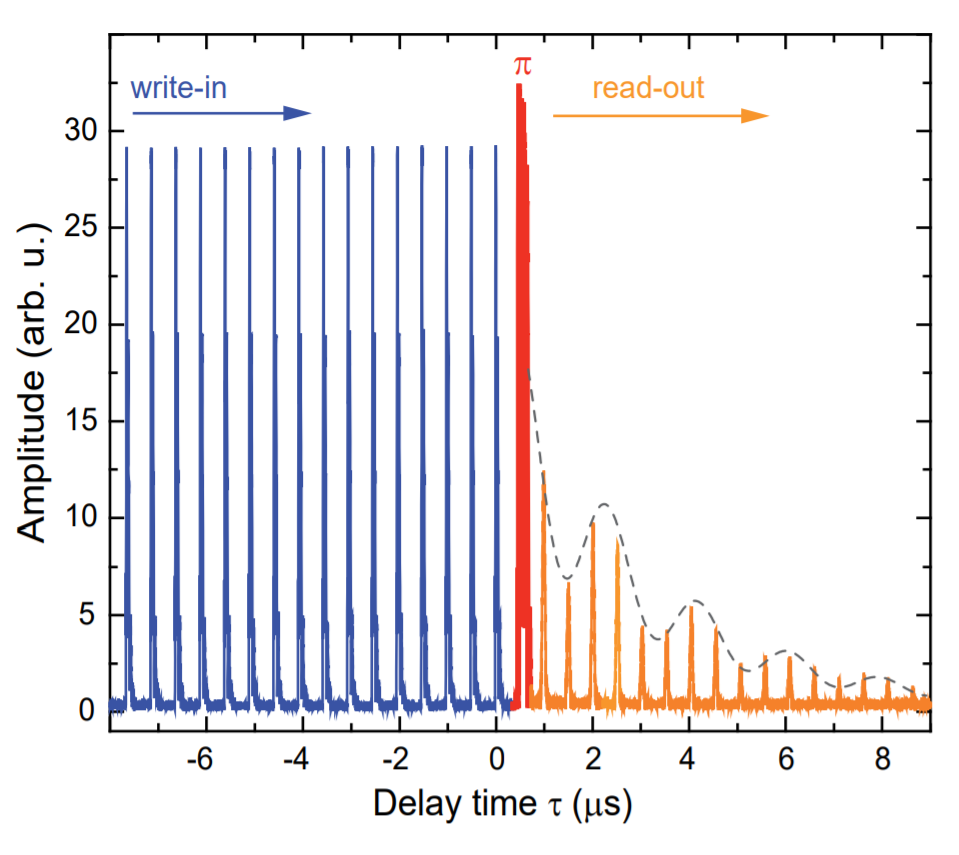
\includegraphics[height=0.4\textwidth,keepaspectratio]{16state}
\caption{\label{fig:16state} Storage of 16 microwave coherent pulses in the high field $S_{2a}$ electronic transition of Eu ions. The grey dashed line is the electron spin echo envelope modulation due to the hyperfine interaction between Y nuclear spins and Eu electronic spins \citep{PhysRevB.92.014421}.}
\end{figure}

Multimode storage and retrieval of 16 weak coherent microwave pulses in a Er$^{3+}$ doped YSO crystal placed on a copper coplanar waveguide is demonstrated at $mK$ temperature in Ref.~\citep{PhysRevB.92.014421}. Collective ensemble encoding for a spin system due to the absorption of a photon is described as:

\begin{equation}
\label{eq:qubit}
\ket{\Psi}_{c} = \frac{1}{\sqrt{N}} \sum_{k=1}^{N}\ket{\downarrow_{1} \downarrow_{2}...\uparrow_{k}...\downarrow_{N}}\exp{-i\delta_{k}t}, 
\end{equation} 

where $\delta_{k}$ is the k-th spin detuning from the average precession frequency of the spin ensemble. Dephasing results in $\ket{\Psi}_{c}$ evolving into a dark mode. Thus another single photon can be absorbed by spins. The number of stored modes, which is 56 for this system, is upper-bounded by $T_{2}/T_{2}^{*}$ where $T_{2}$ is the coherence time and $T_{2}^{*}$ is the dephasing time. The application of the refocusing $\pi$-pulse results in the emission of the microwave pulses is shown in Fig.~\ref{fig:16state} where the output photon emission is reversed with respect to the input photons. The oscillatory behavior of the retrieved pulses is expected to be due to the nuclear spin of Y ions interacting with the RE electronic spins. This additionally indicates that nuclear spin of $^{89}$Y ions has potential for memory applications. In addition, reversible mapping of temporal optical modes using Nd doped YSO with a 883 nm transition wavelength is investigated in Ref.~\citep{Usmani2010MappingMP}. 


\begin{figure}[h]
\centering
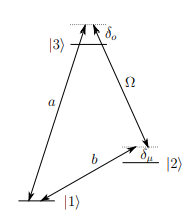
\includegraphics[height=0.4\textwidth,keepaspectratio]{3levelatom}
\caption{\label{fig:3levelatom} Energy level schematic of the Er atoms. The microwave cavity mode is coupled to the spin transition with frequency $\omega_{b}$. The optical cavity mode couples to the $\ket{1}\leftrightarrow \ket{3}$ transition with frequency $\omega_{a}$. There is an additional coherent driving field $\Omega$ for the transition $\ket{2}\leftrightarrow \ket{3}$ ~\citep{PhysRevLett.113.203601}.}
\end{figure}


Reversible mapping of multimode pulses in RE doped substrates is an impressive step towards building a hybrid quantum memory. Conversely, the distributed quantum computing architecture additionally requires the ability to achieve efficient microwave-to-optical conversion to enable long distance transmission of quantum states. In Ref.~\citep{PhysRevLett.113.203601} a theoretical proposal for a 100$\%$ efficient microwave-optical transducer is outlined for a cryogenic Er doped crystal. The crystal is placed inside a microwave and optical resonator where coupling of the Er atoms to the cavities is described in Fig.~\ref{fig:3levelatom}. The three off-resonant fields are detuned such that $\omega_{a} = \omega_{b}+\omega_{\Omega}$. The photons emitted by Er occur at a wavelength compatible with long distance transfer over an optical fiber. For large detuning such that excited atomic states are adiabatically eliminated the Hamiltonian terms describing the coupling between the two modes has a strength, S:

\begin{equation}
\label{eq:qubit}
S = \sum_{k} \frac{\Omega_{k}\nu_{\mu,k} \nu^{*}_{o,k}}{\delta_{o,k}\delta_{\mu,k}}
\end{equation}

where the coupling strengths of $k$-th atom to the microwave and optical resonator is $\nu_{\mu,k}$ and $\nu_{o,k}$ respectively. The coherent driving field has the Rabi frequency $\Omega_{k}$. Therefore to achieve perfect mapping of the microwave field to an optical field the condition $4\left | S \right | = \kappa_{a}\kappa_{b}$ must be satisfied where $\kappa$ describes the cavity decay rate. Thus efficient conversion requires coupling between the Er atoms and one or both of cavities to be in the strong coupling regime. Strong coupling of RE ions to a microwave cavity has been achieved in Ref.~\citep{PhysRevLett.110.157001} as previously discussed and strong coupling to an optical cavity is demonstrated in Ref.~\citep{PhysRevA.74.033818}.      

\begin{figure}[h]
\centering
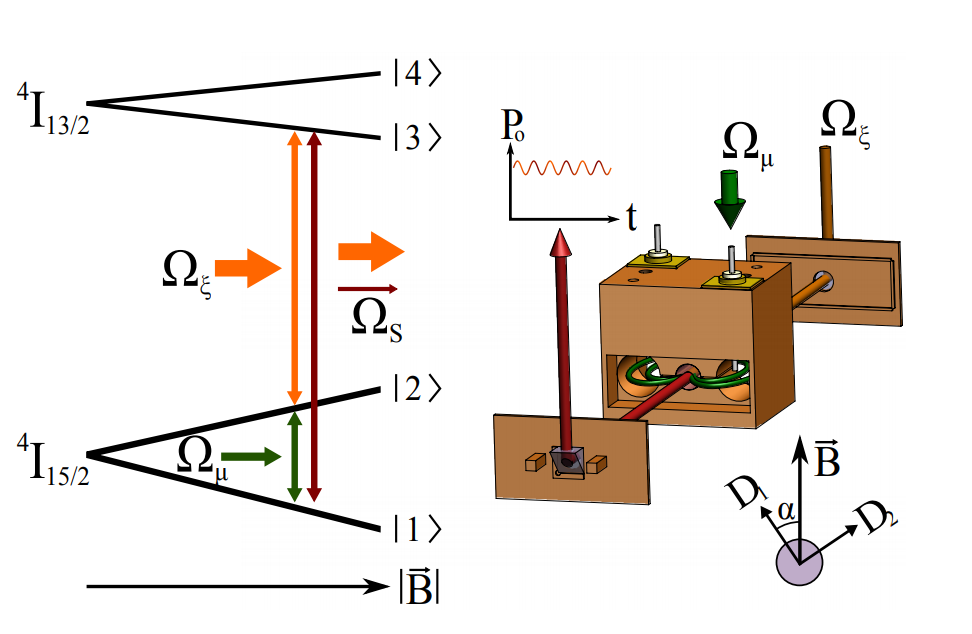
\includegraphics[height=0.4\textwidth,keepaspectratio]{frequencyupconversion}
\caption{\label{fig:frequencyupconversion} (Left) The optical transition is obtained between the $^{4}$I$_{15/2}$ and $^{4}$I$_{13/2}$ energy levels of Er doped YSO which is driven by the $\Omega_{\xi}$. The application an external field magnetic field results in the $^{4}$I$_{15/2}$ electron spin resonance being driven by the $\Omega_{\mu}$ field. The resulting optical field is $\Omega_{s}$. (Right) The experimental schematic where the sample resides inside the loop-gap resonator where the dielectric axis of the crystal with respect to input microwave fields is shown. Light is transmitted to or from the sample using via a prism pair ~\citep{PhysRevA.92.062313}.}
\end{figure}

Experimental demonstration of microwave-to-optical conversion using an Er doped YSO sample is presented in Ref.~\citep{PhysRevA.92.062313}. The experimental setup and coupling transitions are shown in Fig.~\ref{fig:frequencyupconversion}. The input microwave and optical field generate a coherence between $\ket{1} \rightarrow \ket{3}$ where using the Raman heterodyne spectroscopy scheme, the output of this field is detected through the beat note of the optical coupling beam. The low efficiency of the conversion is expected to be improved by the addition of an optical resonator to increase the coupling strength.  

To summarise recent investigations of RE doped YSO illustrates the exciting potential of this system to provide a quantum memory of a hybrid distributed quantum computing architecture. The experimental schemes discussed here highlight that RE ions can achieve strong coupling to microwave and optical cavities which is a crucial requirement for a quantum transducer protocols. Additionally storage and retrieval of multimode microwave pulses is an initial impressive step towards building a quantum memory, where the ultimate goal is reversible, high-efficiency quantum state transfer between disparate qubits.



\section{The effect of strain in hybrid quantum systems}
The motivation for this project arises due to the interest in coupling RE doped YSO to superconducting resonators using the flip-chip approach~\citep{PhysRevLett.110.157001} or direct metal deposition~\citep{doi:10.1063/1.4894455}. The requirement of cryogenic temperatures for operation is expected to induce strain in the crystal environment. This effect is due to difference in thermal expansion coefficients for the substrates and thus could produce a perturbation of the spin distribution. Similarly, this a concern for donor spins in silicon where superconducting resonators are patterned onto the sample~\citep{doi:10.1063/1.4919761}. 

The expected cause of the observed variation from the bulk properties for nano-fabricated electronic substrates on donor spin doped Si substrates was due to induced electric fields or strain effects~\citep{10.1038/NNANO.2014.211}. Investigation of resonance shifts of three aluminum superconducting resonators pattered on the surface of a 700 nm isotropically purified $^{28}$Si substrate with implanted $^{209}$Bi donors~\citep{PhysRevApplied.9.044014}.Electron paramagnetic resonance (EPR) spectroscopy completed on the $\ket{F=4,m_{F}=-4} \leftrightarrow \ket{F=5,m_{F}=-5}$ transition, where $\Delta m_{F} = \pm 1$. This reveals transition peak splitting each with a 100 $\mu$T linewidth compared to single 20 $\mu$ peak measured in the absence of a patterned superconducting resonator as shown in Fig.~\ref{fig:straininducedsplitting}. 


\begin{figure}[h]
\centering
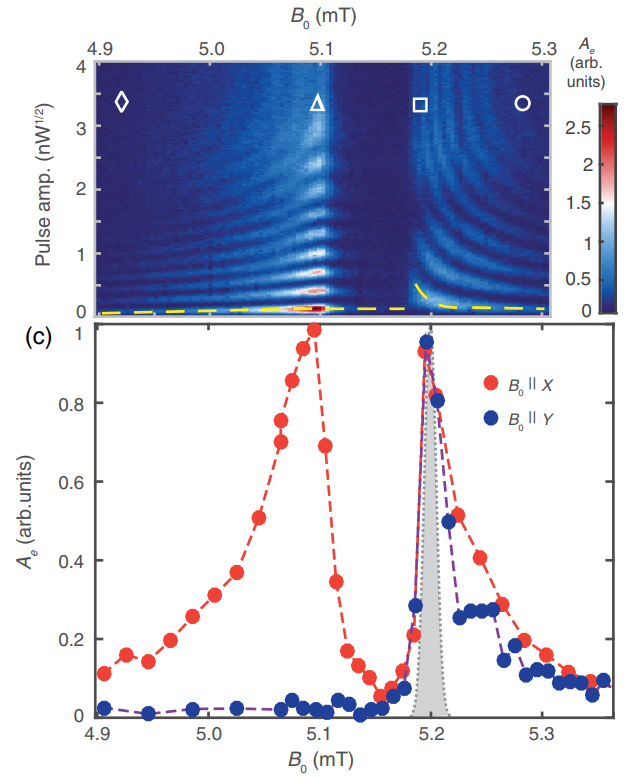
\includegraphics[height=0.45\textwidth,keepaspectratio]{straininducedsplitting}
\caption{\label{fig:straininducedsplitting} The echo signal detected using the Hahn echo sequence for the $\ket{F=4,m_{F}=-4} \leftrightarrow \ket{F=5,m_{F}=-5}$ for $B_{0} \parallel X$ (red) and $B_{0} \parallel Y$ (blue). The grey curve shows the peak transition for the system with no on-chip resonator ~\citep{PhysRevApplied.9.044014}.}
\end{figure}


The low peak observed for  vanishes for $B_{0} \parallel X$ vanishes for $B_{0} \parallel Y$ which is attributed to the condition $\delta B_{1}\perp B_{0}$ for excitation, where $\delta B_{1}$ is the magnetic field vacuum fluctuations in the resonator. Directly under an electrode, of the interdigited LC resonator, dominated by $\delta B_{1Y}$ with contribution of $\delta B_{1Z}$ to the side of the electrode. Therefore, only $\delta B_{1z}$ contributes for $B_{0} \parallel Y$. Further investigation of spin transitions discounts an in-built electric field or magnetic field inhomogeneity as the mechanism for the splitting and broadening of the transition peak. Therefore upon consideration of strain, this mechanism has the ability to modify the electron spin (S=1/2) and nuclear spin (I=9/2) transitions for $^{209}$Bi. Strain can modify the quadrupole interaction, the hyperfine interaction strength $A$ and the electron g-factor.   

The quadrupole interaction arises due to axial symmetry of the nuclear charge distribution where nuclear quadrupole moment $Q$ describes the degree of deformation from spherical charge distribution. The non-spherical nucleus interact with nearby electrons resulting in an electrostatic field gradient $V_{ab}$ at the nucleus where $a$ and $b$ are the local crystal frame principle axes. The Hamiltonian term for the quadrupole interaction is thus:

\begin{equation}
\label{eq:quadropleinteraction}
H_{Q} = \frac{e V_{zz} Q}{4I(2I-1)}\left [3I^{2}_{z}-I^{2}+\eta (I^{2}_{x} - I^{2}_{y} \right ],
\end{equation} 

where the asymmetry parameter is $\eta = (V_{xx}-V_{yy}/V{zz}$ and the electron charge is $e$~\citep{Suits2006}. Ref.~\citep{PhysRevLett.115.057601} demonstrates that the quadrupole interaction can be manipulated by strain applied to Si doped with As$^{+}$ ions using piezo-actuators. The induced strain can be used to tune the nuclear spin properties of As$^{+}$ ions. For the unstrained sample the cubic crystal symmetry cancels out the electric field gradients whilst applying uniaxial strain mimics the effect of strain induced at mK temperatures for substrates with different thermal expansion coefficients and results in a nonzero electric field gradient. 

\begin{figure}[H]
    \centering
    \begin{subfigure}[b]{0.6\textwidth}
        \centering
        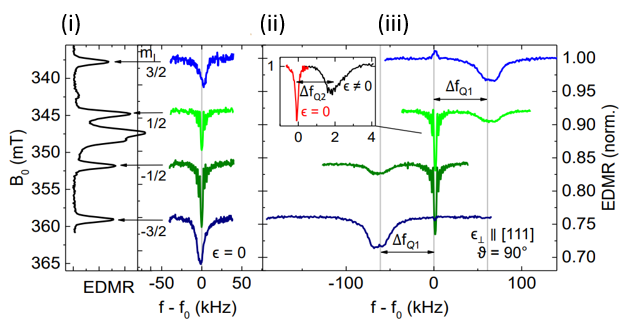
\includegraphics[width=\textwidth]{nuclearshifts}
        \caption{\label{fig:nuclearshifts}(i) electrically detected
magnetic resonance (EDMR) spectrum for As$^{0}$ in Si. (ii) unstrained NMR transitions for As$^{+}$ in Si. (iii) strained NMR transitions for A$^{+}$. The insert shows the $\ket{m_{I}=1/2} \leftrightarrow \ket{-1/2} $ transitions in high-resolution~\citep{PhysRevLett.115.057601}.}
    \end{subfigure}
        \begin{subfigure}[b]{0.6\textwidth}
        \centering
        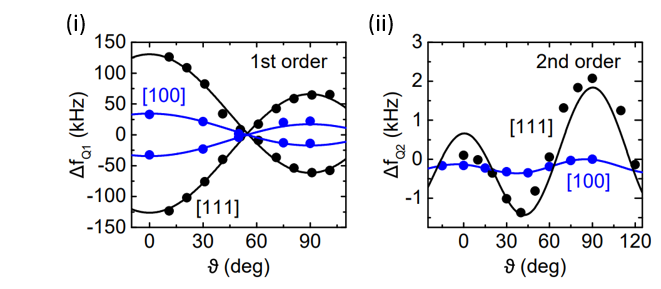
\includegraphics[width=\textwidth]{nuclearshifts2}
        \caption{\label{fig:nuclearshifts2} Angular dependence of (i) first-order and (ii) second-order resonance frequency shifts dependent on the magnetic field orientation where the electric field gradient generated in [111] and [100] crystal directions~\citep{PhysRevLett.115.057601}.}
    \end{subfigure}
    \caption{}
\label{fig:}
\end{figure}

Comparison of the unaxial strain of the order of 10$^{-4}$ and unstrained nuclear magnetic resonance (NMR) spectrum probed using 9.74 GHz resonator is shown in Fig.~\ref{fig:nuclearshifts}. This reveals outer transitions (ie $\ket{m_{I}=3/2} \leftrightarrow \ket{1/2}$ and $\ket{-3/2} \leftrightarrow \ket{-1/2}$ have a resonance shift greater than the resonance linewidth described by the first order frequency shift. Additionally for these transitions asymmetric broadening is observed in absence of the piezo-mechanical strain and is attributed to strain induced by the contact. Conversely only a small second order frequency shift is observed for the sharp $\ket{1/2} \leftrightarrow \ket{-1/2}$ resonance. Further investigation using long rf-pulses as shown in the insert of Fig.~\ref{fig:nuclearshifts} determines that the inner transition is similarly shifted by more than one linewidth but due to the difference in linewidth, between the inner and outer transition, the shift is significantly smaller. Fig.~\ref{fig:nuclearshifts2} presents a characterisation of the resonance shift due to anisotropic electric field gradient as a function of angle $\vartheta$ between magnetic field and strain axis. The quadrupole shift is related to the applied strain through the a tensor $S_{ij}$ with nonzero $S_{11}$ and $S_{44}$ components. However, comparison of $df/dQ$ sensitivity to EPR transitions it is clear the quadrupole interaction is not the origin of the resonance splitting~\citep{PhysRevApplied.9.044014}.

The study of strain induced resonance frequency shifts due to perturbation of the hyperfine coupling of group V donor spins in $^{28}$Si is completed~\citep{PhysRevLett.120.167701}. The compressive strain is applied using masses placed on top of the sample and is expected to modify the band structure of Si. Thus the valley repopulation model (VRM)~\citep{PhysRev.124.1068} was utilised to understand the effect of Si crystal symmetry breaking which lifts the Si six valley degeneracy. Strain induces mixing of the donor singlet $A_{1}$ ground state and the doublet $E$ excited state. The hyperfine interaction Hamiltonian term is presented in Section.~\ref{sec:hyperfine} where the isotropic hyperfine interaction strength $A$ is given in Eq.~\ref{eq:hyperfinestrength}. The EPR transitions of $^{209}$Bi doped in Si, the sample mount and observed shift in resonance frequency due to small (10$^{-5}$) strain is shown in Fig.~\ref{fig:mansirpaper}. 

\begin{figure}[h]
\centering
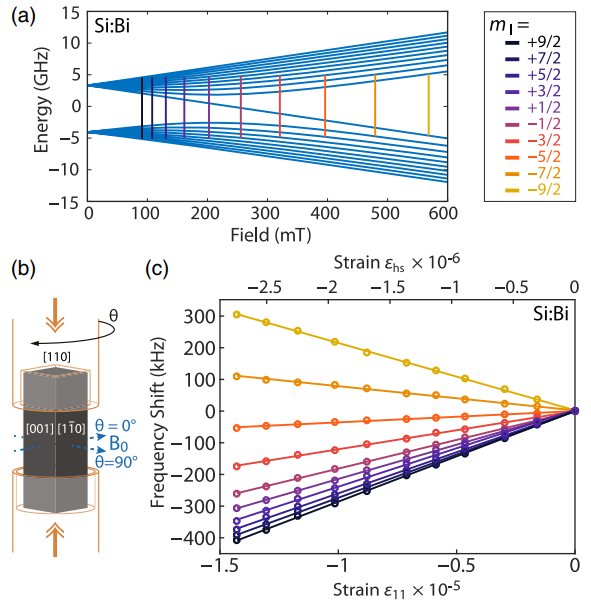
\includegraphics[height=0.45\textwidth,keepaspectratio]{mansirpaper}
\caption{\label{fig:mansirpaper} (a) $^{209}$Bi (S=1/2, I=9/2) doped in Si EPR spectrum. (b) Mechanical strian experimental setup where $\theta$ is orientation of $B_{0}$ with respect to the [001] crystal axis. (c) Observed linear EPR frequency shifts as a function of the strain $\epsilon_{11}$ for $\theta = 30^{\circ}$ ~\citep{PhysRevLett.120.167701}.}
\end{figure}

The VRM model predicts quadratic shift of $A$ for the application of unaxial strain. However, the observed linear shift is attributed to uniaxial stress applied to the crystal producing three linear strain components, $\epsilon_{11}$, $\epsilon_{22}$ and $\epsilon_{33}$ where the hydrostatic strain mechanism is described as $\epsilon_{hs} = (\epsilon_{11}+\epsilon_{22}+\epsilon_{33}/2$). Comparison of isotropic hyperfine coupling $df/dA$ to the experimentally measured $df/d\epsilon_{11}$ determines the linear strain mechanism dominates. The tight binding (TB) model~\citep{PhysRevB.79.245201} describing the variation of bound states $Bi$ doped Si under strain provides a good agreement for small applied strain with experimentally. The determined relationship $A/A_{0}$ where $A_{0}$ is the unstrained hyperfine interaction strength to second order the strain is:

\begin{equation}
\label{eq:Atermmodel}
A(\bm{\epsilon})/A_{0} = 1+\frac{K}{3}(\epsilon_{xx}+\epsilon_{yy}+\epsilon_{zz})+\frac{L}{2}\left [ (\epsilon_{yy}-epsilon_{zz})^{2}+(\epsilon_{xx}-\epsilon_{zz})^{2}+(\epsilon_{xx}-\epsilon_{yy})^{2}) \right ] +N(\epsilon^{2}_{yz}+\epsilon^{2}_{xz}+\epsilon^{2}_{xy}),
\end{equation} 

where A fit to the TB model obtains K = 29.3, L = -9064 and N = -225. Additionally, investigation the induced anisotropy of the g-tensor for V group donors in Si is fitted to a model developed which contains a VRM term and the spin-orbit coupling term. Applying the model in Eq.~\ref{eq:Atermmodel} to the Si doped As$^{+}$ device with LC resonator pattered on the surface in Ref.~\citep{PhysRevApplied.9.044014} determines $A(\bm{\epsilon})=$ 1MHz for strain of the order of 10$^{-4}$. This results in a resonance shift in agreement with the experimentally measured result of Fig.~\ref{fig:straininducedsplitting}. Therefore the strain induced modification of the $A$ is determined to be the resonance peak splitting mechanism. 


\begin{figure}[h]
\centering
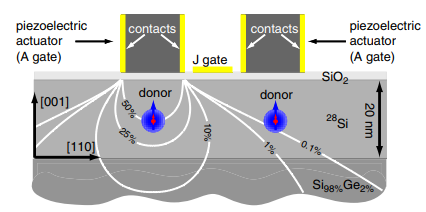
\includegraphics[height=0.45\textwidth,keepaspectratio]{piezoelectric}
\caption{\label{fig:piezoelectric} The schematic of the piezoelectric actuators which can apply strain to the $^{28}$Si substrate in locations of a donor spin. This device tunes the coupling strength between the nuclear and electronic spin of the P donor. The distribution of the out of plane strain is illustrated using isolines is modelled using density function theory calculations. To maximise the effect of the nanoactuators $^{28}$Si is grown on a SiGe substrate ~\citep{PhysRevLett.106.037601}.}
\end{figure}

The applications of the strain induced ability to shift a resonance peak of a spin system by more than a linewidth does not go unnoticed \citep{PhysRevLett.120.167701,PhysRevApplied.9.044014,PhysRevLett.115.057601}. The scheme to Stark tune the hyperfine interaction of P doped Si using piezoelectric nanoactuators is illustrated in Fig.~\ref{fig:piezoelectric}. This scheme provides a 17 $\mu$T shift of the P hyperfine transitions with a 8 $\mu$T linewidth. Therefore, this device has potential to provide an additional degree of freedom to tune qubits in and out of resonance. Additionally, in Ref.~\citep{PhysRevB.88.064308} applying mechanical stress to a single acceptor in a patterned Si substrate is shown to partially lift the ground state degeneracy. In the presence of strain in addition to the magnetic field the qubit can decoupled to the first order decoupled from the acoustic phonons used to coherently manipulate the state of the qubit.   

The theoretical treatment of the interaction between the applied strain and electron spin of NV centers is presented in Ref.~\citep{PhysRevB.98.075201}. This study suggests that magnetically forbidden transitions, in addition to allowed transition, can be coherently driven using mechanically deforming the crystal at a rate equal to the Rabi frequency. In Ref.~\citep{PhysRevLett.111.227602} the ground state Hamiltonian of the spin system is given as:

\begin{equation}
\label{eq:HamiltonianNV}
H_{NV} = D_{0}S^{2}_{z}+\gamma_{NV}B_{\parallel}S_{z}+\gamma_{NV}B_{\perp}S_{x}+\epsilon_{\perp} \left | \sigma_{x}(S_{x}S_{y}+S_{y}S_{x})+\sigma_{y}(S^{2}_{x}-S^{2}_{y}) \right |, 
\end{equation} 

where $D_{0}$ and $\gamma_{NV}$ is the zero-field splitting and the gyromagnetic ratio, respectively. The degeneracy of the $\ket{m_{s}=0}$ and $\ket{\pm 1}$ is lift by $D_{0}$. The components of the magnetic field are given as $B_{\parallel}$ and $B_{\perp}$ and the components of the electron spin operator as $S_{x},S_{y} and S_{z}$ where z-axis is along the crystal's symmetry axis. Alignment of $B_{\parallel}$ splits the degeneracy of $\ket{+1}$ and $\ket{-1}$. Coherent driving of $\ket{0} \leftrightarrow \ket{\pm 1}$ is achieved by an oscillating $B_{\perp}$ field. The addition of a GHz stress perpendicular to the symmetry axis drives the magnetically forbidden spin transition $\ket{-1} \leftrightarrow \ket{+1}$. Thus addition of mechanical strain enables driving between all the spin states. A bulk acoustic resonator is used to generate the stress resonant with the $\ket{-1} \leftrightarrow \ket{+1}$ transition where the magnetic spin resonance is achieved using an optical detection scheme at room temperature. Moreover, in Ref.~\citep{2040-8986-19-4-044003} decoupling from the environmental noise is achieved by driving the spin transitions with a mechanical oscillator. The coherence time of the qubit is increased by two orders of magnitude.  
    
